% Created by tikzDevice version 0.12.3.1 on 2023-05-05 12:22:56
% !TEX encoding = UTF-8 Unicode
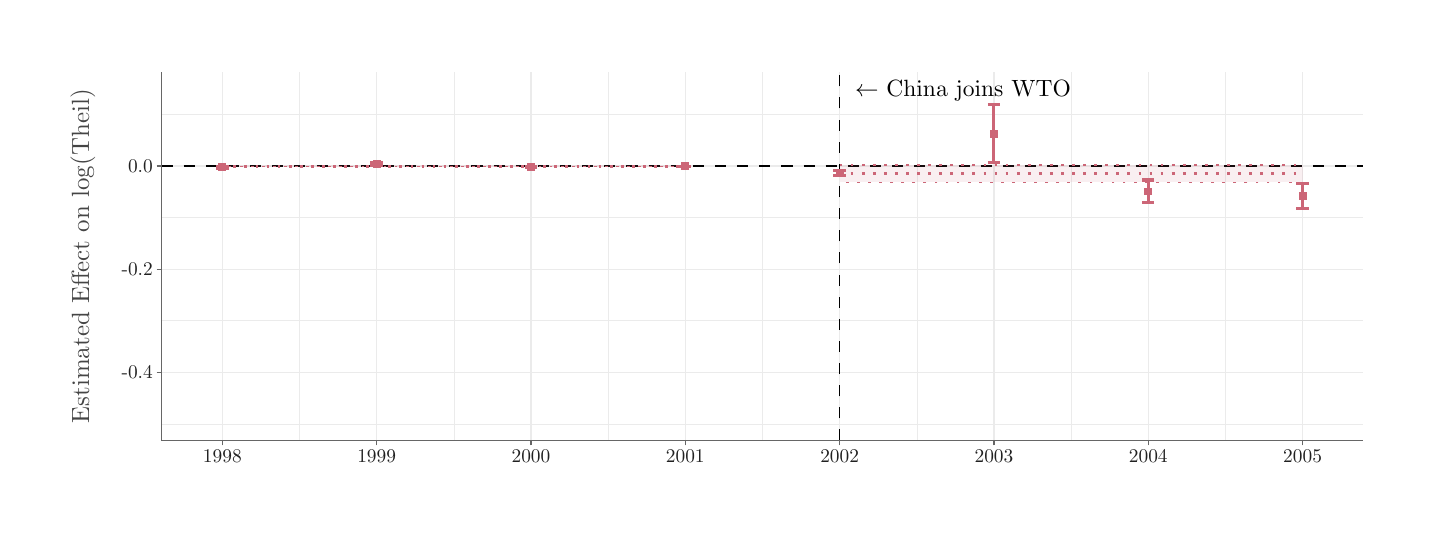
\begin{tikzpicture}[x=1pt,y=1pt]
\definecolor{fillColor}{RGB}{255,255,255}
\path[use as bounding box,fill=fillColor,fill opacity=0.00] (0,0) rectangle (498.66,174.53);
\begin{scope}
\path[clip] (  0.00,  0.00) rectangle (498.66,174.53);
\definecolor{fillColor}{RGB}{255,255,255}

\path[fill=fillColor] (  0.00,  0.00) rectangle (498.66,174.53);
\end{scope}
\begin{scope}
\path[clip] ( 48.37, 25.33) rectangle (482.66,158.53);
\definecolor{fillColor}{RGB}{255,255,255}

\path[fill=fillColor] ( 48.37, 25.33) rectangle (482.66,158.53);
\definecolor{drawColor}{gray}{0.92}

\path[draw=drawColor,line width= 0.2pt,line join=round] ( 48.37, 31.39) --
	(482.66, 31.39);

\path[draw=drawColor,line width= 0.2pt,line join=round] ( 48.37, 68.65) --
	(482.66, 68.65);

\path[draw=drawColor,line width= 0.2pt,line join=round] ( 48.37,105.90) --
	(482.66,105.90);

\path[draw=drawColor,line width= 0.2pt,line join=round] ( 48.37,143.16) --
	(482.66,143.16);

\path[draw=drawColor,line width= 0.2pt,line join=round] ( 98.22, 25.33) --
	( 98.22,158.53);

\path[draw=drawColor,line width= 0.2pt,line join=round] (153.99, 25.33) --
	(153.99,158.53);

\path[draw=drawColor,line width= 0.2pt,line join=round] (209.75, 25.33) --
	(209.75,158.53);

\path[draw=drawColor,line width= 0.2pt,line join=round] (265.52, 25.33) --
	(265.52,158.53);

\path[draw=drawColor,line width= 0.2pt,line join=round] (321.28, 25.33) --
	(321.28,158.53);

\path[draw=drawColor,line width= 0.2pt,line join=round] (377.04, 25.33) --
	(377.04,158.53);

\path[draw=drawColor,line width= 0.2pt,line join=round] (432.81, 25.33) --
	(432.81,158.53);

\path[draw=drawColor,line width= 0.4pt,line join=round] ( 48.37, 50.02) --
	(482.66, 50.02);

\path[draw=drawColor,line width= 0.4pt,line join=round] ( 48.37, 87.27) --
	(482.66, 87.27);

\path[draw=drawColor,line width= 0.4pt,line join=round] ( 48.37,124.53) --
	(482.66,124.53);

\path[draw=drawColor,line width= 0.4pt,line join=round] ( 70.34, 25.33) --
	( 70.34,158.53);

\path[draw=drawColor,line width= 0.4pt,line join=round] (126.10, 25.33) --
	(126.10,158.53);

\path[draw=drawColor,line width= 0.4pt,line join=round] (181.87, 25.33) --
	(181.87,158.53);

\path[draw=drawColor,line width= 0.4pt,line join=round] (237.63, 25.33) --
	(237.63,158.53);

\path[draw=drawColor,line width= 0.4pt,line join=round] (293.40, 25.33) --
	(293.40,158.53);

\path[draw=drawColor,line width= 0.4pt,line join=round] (349.16, 25.33) --
	(349.16,158.53);

\path[draw=drawColor,line width= 0.4pt,line join=round] (404.93, 25.33) --
	(404.93,158.53);

\path[draw=drawColor,line width= 0.4pt,line join=round] (460.69, 25.33) --
	(460.69,158.53);
\definecolor{drawColor}{RGB}{0,0,0}

\path[draw=drawColor,line width= 0.6pt,dash pattern=on 4pt off 4pt ,line join=round] ( 48.37,124.53) -- (482.66,124.53);

\path[draw=drawColor,line width= 0.6pt,dash pattern=on 4pt off 4pt ,line join=round] (293.40, 25.33) -- (293.40,158.53);

\node[text=drawColor,anchor=base west,inner sep=0pt, outer sep=0pt, scale=  0.85] at (298.97,149.54) {$\leftarrow$ China joins WTO};
\definecolor{drawColor}{RGB}{204,102,119}

\path[draw=drawColor,line width= 1.1pt,line join=round] ( 68.11,124.48) --
	( 72.57,124.48);

\path[draw=drawColor,line width= 1.1pt,line join=round] ( 70.34,124.48) --
	( 70.34,123.78);

\path[draw=drawColor,line width= 1.1pt,line join=round] ( 68.11,123.78) --
	( 72.57,123.78);

\path[draw=drawColor,line width= 1.1pt,line join=round] (123.87,125.90) --
	(128.34,125.90);

\path[draw=drawColor,line width= 1.1pt,line join=round] (126.10,125.90) --
	(126.10,124.64);

\path[draw=drawColor,line width= 1.1pt,line join=round] (123.87,124.64) --
	(128.34,124.64);

\path[draw=drawColor,line width= 1.1pt,line join=round] (179.64,124.49) --
	(184.10,124.49);

\path[draw=drawColor,line width= 1.1pt,line join=round] (181.87,124.49) --
	(181.87,124.03);

\path[draw=drawColor,line width= 1.1pt,line join=round] (179.64,124.03) --
	(184.10,124.03);

\path[draw=drawColor,line width= 1.1pt,line join=round] (235.40,124.53) --
	(239.86,124.53);

\path[draw=drawColor,line width= 1.1pt,line join=round] (237.63,124.53) --
	(237.63,124.43);

\path[draw=drawColor,line width= 1.1pt,line join=round] (235.40,124.43) --
	(239.86,124.43);

\path[draw=drawColor,line width= 1.1pt,line join=round] (291.17,122.86) --
	(295.63,122.86);

\path[draw=drawColor,line width= 1.1pt,line join=round] (293.40,122.86) --
	(293.40,121.04);

\path[draw=drawColor,line width= 1.1pt,line join=round] (291.17,121.04) --
	(295.63,121.04);

\path[draw=drawColor,line width= 1.1pt,line join=round] (346.93,146.71) --
	(351.39,146.71);

\path[draw=drawColor,line width= 1.1pt,line join=round] (349.16,146.71) --
	(349.16,125.75);

\path[draw=drawColor,line width= 1.1pt,line join=round] (346.93,125.75) --
	(351.39,125.75);

\path[draw=drawColor,line width= 1.1pt,line join=round] (402.70,119.48) --
	(407.16,119.48);

\path[draw=drawColor,line width= 1.1pt,line join=round] (404.93,119.48) --
	(404.93,111.19);

\path[draw=drawColor,line width= 1.1pt,line join=round] (402.70,111.19) --
	(407.16,111.19);

\path[draw=drawColor,line width= 1.1pt,line join=round] (458.46,118.36) --
	(462.92,118.36);

\path[draw=drawColor,line width= 1.1pt,line join=round] (460.69,118.36) --
	(460.69,109.08);

\path[draw=drawColor,line width= 1.1pt,line join=round] (458.46,109.08) --
	(462.92,109.08);
\definecolor{fillColor}{RGB}{204,102,119}

\path[fill=fillColor] ( 68.91,122.70) --
	( 71.77,122.70) --
	( 71.77,125.55) --
	( 68.91,125.55) --
	cycle;

\path[fill=fillColor] (124.68,123.84) --
	(127.53,123.84) --
	(127.53,126.70) --
	(124.68,126.70) --
	cycle;

\path[fill=fillColor] (180.44,122.83) --
	(183.30,122.83) --
	(183.30,125.69) --
	(180.44,125.69) --
	cycle;

\path[fill=fillColor] (236.21,123.05) --
	(239.06,123.05) --
	(239.06,125.90) --
	(236.21,125.90) --
	cycle;

\path[fill=fillColor] (291.97,120.52) --
	(294.82,120.52) --
	(294.82,123.37) --
	(291.97,123.37) --
	cycle;

\path[fill=fillColor] (347.74,134.81) --
	(350.59,134.81) --
	(350.59,137.66) --
	(347.74,137.66) --
	cycle;

\path[fill=fillColor] (403.50,113.91) --
	(406.35,113.91) --
	(406.35,116.76) --
	(403.50,116.76) --
	cycle;

\path[fill=fillColor] (459.27,112.29) --
	(462.12,112.29) --
	(462.12,115.14) --
	(459.27,115.14) --
	cycle;
\definecolor{fillColor}{RGB}{204,102,119}

\path[fill=fillColor,fill opacity=0.10] (293.40,125.01) --
	(460.69,125.01) --
	(460.69,118.60) --
	(293.40,118.60) --
	cycle;

\path[draw=drawColor,line width= 0.6pt,dash pattern=on 1pt off 3pt ,line join=round] (293.40,125.01) --
	(460.69,125.01);

\path[draw=drawColor,line width= 0.6pt,dash pattern=on 1pt off 3pt ,line join=round] (460.69,118.60) --
	(293.40,118.60);

\path[fill=fillColor,fill opacity=0.10] ( 70.34,124.73) --
	(237.63,124.73) --
	(237.63,124.34) --
	( 70.34,124.34) --
	cycle;

\path[draw=drawColor,line width= 0.6pt,dash pattern=on 1pt off 3pt ,line join=round] ( 70.34,124.73) --
	(237.63,124.73);

\path[draw=drawColor,line width= 0.6pt,dash pattern=on 1pt off 3pt ,line join=round] (237.63,124.34) --
	( 70.34,124.34);

\path[draw=drawColor,line width= 1.1pt,dash pattern=on 1pt off 3pt ,line join=round] (293.40,121.81) --
	(460.69,121.81);

\path[draw=drawColor,line width= 1.1pt,dash pattern=on 1pt off 3pt ,line join=round] ( 70.34,124.53) --
	(237.63,124.53);
\end{scope}
\begin{scope}
\path[clip] (  0.00,  0.00) rectangle (498.66,174.53);
\definecolor{drawColor}{gray}{0.40}

\path[draw=drawColor,line width= 0.4pt,line join=round] ( 48.37, 25.33) --
	( 48.37,158.53);
\end{scope}
\begin{scope}
\path[clip] (  0.00,  0.00) rectangle (498.66,174.53);
\definecolor{drawColor}{gray}{0.13}

\node[text=drawColor,anchor=base east,inner sep=0pt, outer sep=0pt, scale=  0.70] at ( 45.22, 47.61) {-0.4};

\node[text=drawColor,anchor=base east,inner sep=0pt, outer sep=0pt, scale=  0.70] at ( 45.22, 84.86) {-0.2};

\node[text=drawColor,anchor=base east,inner sep=0pt, outer sep=0pt, scale=  0.70] at ( 45.22,122.12) {0.0};
\end{scope}
\begin{scope}
\path[clip] (  0.00,  0.00) rectangle (498.66,174.53);
\definecolor{drawColor}{gray}{0.40}

\path[draw=drawColor,line width= 0.4pt,line join=round] ( 46.62, 50.02) --
	( 48.37, 50.02);

\path[draw=drawColor,line width= 0.4pt,line join=round] ( 46.62, 87.27) --
	( 48.37, 87.27);

\path[draw=drawColor,line width= 0.4pt,line join=round] ( 46.62,124.53) --
	( 48.37,124.53);
\end{scope}
\begin{scope}
\path[clip] (  0.00,  0.00) rectangle (498.66,174.53);
\definecolor{drawColor}{gray}{0.40}

\path[draw=drawColor,line width= 0.4pt,line join=round] ( 48.37, 25.33) --
	(482.66, 25.33);
\end{scope}
\begin{scope}
\path[clip] (  0.00,  0.00) rectangle (498.66,174.53);
\definecolor{drawColor}{gray}{0.40}

\path[draw=drawColor,line width= 0.4pt,line join=round] ( 70.34, 23.58) --
	( 70.34, 25.33);

\path[draw=drawColor,line width= 0.4pt,line join=round] (126.10, 23.58) --
	(126.10, 25.33);

\path[draw=drawColor,line width= 0.4pt,line join=round] (181.87, 23.58) --
	(181.87, 25.33);

\path[draw=drawColor,line width= 0.4pt,line join=round] (237.63, 23.58) --
	(237.63, 25.33);

\path[draw=drawColor,line width= 0.4pt,line join=round] (293.40, 23.58) --
	(293.40, 25.33);

\path[draw=drawColor,line width= 0.4pt,line join=round] (349.16, 23.58) --
	(349.16, 25.33);

\path[draw=drawColor,line width= 0.4pt,line join=round] (404.93, 23.58) --
	(404.93, 25.33);

\path[draw=drawColor,line width= 0.4pt,line join=round] (460.69, 23.58) --
	(460.69, 25.33);
\end{scope}
\begin{scope}
\path[clip] (  0.00,  0.00) rectangle (498.66,174.53);
\definecolor{drawColor}{gray}{0.13}

\node[text=drawColor,anchor=base,inner sep=0pt, outer sep=0pt, scale=  0.70] at ( 70.34, 17.36) {1998};

\node[text=drawColor,anchor=base,inner sep=0pt, outer sep=0pt, scale=  0.70] at (126.10, 17.36) {1999};

\node[text=drawColor,anchor=base,inner sep=0pt, outer sep=0pt, scale=  0.70] at (181.87, 17.36) {2000};

\node[text=drawColor,anchor=base,inner sep=0pt, outer sep=0pt, scale=  0.70] at (237.63, 17.36) {2001};

\node[text=drawColor,anchor=base,inner sep=0pt, outer sep=0pt, scale=  0.70] at (293.40, 17.36) {2002};

\node[text=drawColor,anchor=base,inner sep=0pt, outer sep=0pt, scale=  0.70] at (349.16, 17.36) {2003};

\node[text=drawColor,anchor=base,inner sep=0pt, outer sep=0pt, scale=  0.70] at (404.93, 17.36) {2004};

\node[text=drawColor,anchor=base,inner sep=0pt, outer sep=0pt, scale=  0.70] at (460.69, 17.36) {2005};
\end{scope}
\begin{scope}
\path[clip] (  0.00,  0.00) rectangle (498.66,174.53);
\definecolor{drawColor}{gray}{0.27}

\node[text=drawColor,rotate= 90.00,anchor=base,inner sep=0pt, outer sep=0pt, scale=  0.90] at ( 22.20, 91.93) {Estimated Effect on $\log($Theil$)$};
\end{scope}
\end{tikzpicture}
